\section{Технологический стек}
%
%\begin{frame}
%\frametitle{Задачи выбора стека технологий}
%\begin{enumerate}
%    \item Реализация программного кода
%    \item Хранение данных
%    \item Развертывание
%    \item Тестирование
%    \item Логирование
%    \item Документация
%    \item Протоколы взаимодействия
%\end{enumerate}
%\end{frame}

\begin{frame}
\frametitle{Технологический стек}
\begin{itemize}
    \item Операционная система \textit{Ubuntu 20.04 LTS}
    \item Язык программирования \textit{Python 3.8.12}
    \item База данных \textit{PostgreSQL 12} с расширением \textit{PostGIS 3.1}
    \item Веб-сервер \textit{nginx}
    \item Автоматическое развертывание \textit{Gitlab-CI}
    \item Контейнеризация \textit{Docker} и \textit{docker-compose}
    \item Документация \textit{OpenAPI} и \textit{LaTex}
    \item Система сборки логов \textit{ELK}
    \item Протоколы взаимодействия \textit{REST API over HTTP}
    \item Формат данных \textit{JSON}
\end{itemize}
\end{frame}


\section{Системная архитектура}

\begin{frame}
\frametitle{Общий вид системы}
\begin{figure}
    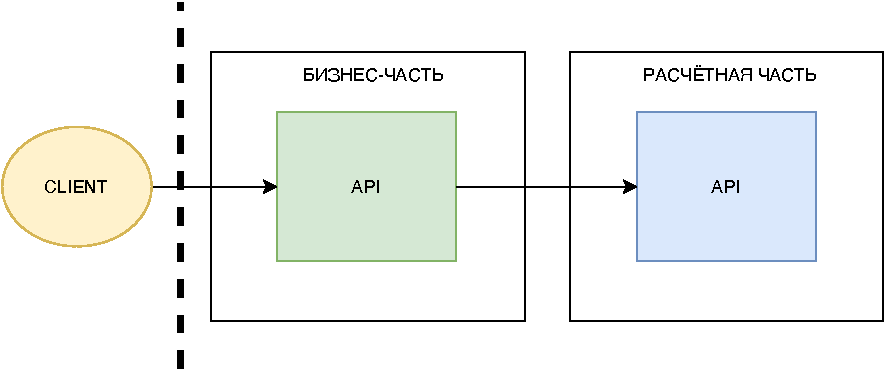
\includegraphics[scale=.9]{pictures/architecture/system}
\end{figure}
\end{frame}

\begin{frame}
\frametitle{Компоненты расчётной части системы}
\begin{figure}
    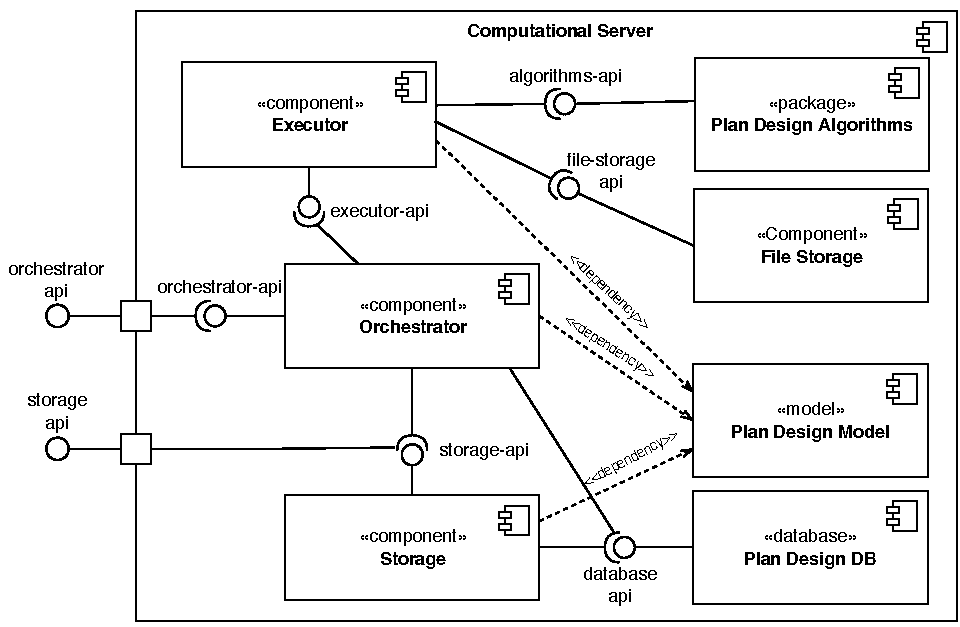
\includegraphics[scale=.6]{pictures/architecture/component}
\end{figure}
\end{frame}

\begin{frame}
\frametitle{Сервис запуска математических методов}
\begin{figure}
    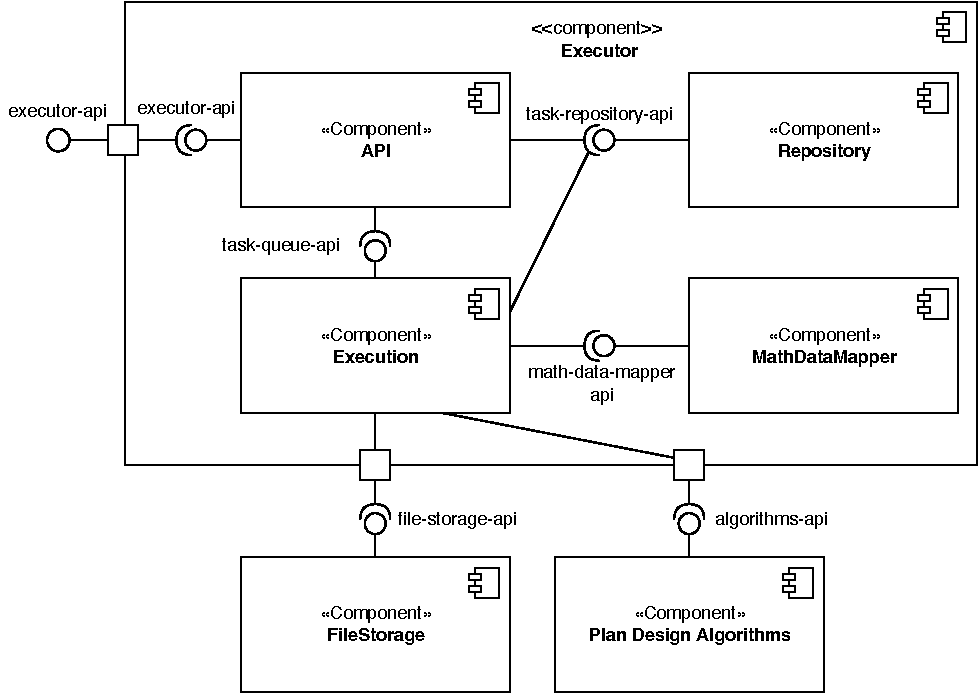
\includegraphics[scale=.6]{pictures/architecture/executor_component_common}
\end{figure}
\end{frame}

\begin{frame}
\frametitle{Компонент запуска математических методов}
\begin{figure}
    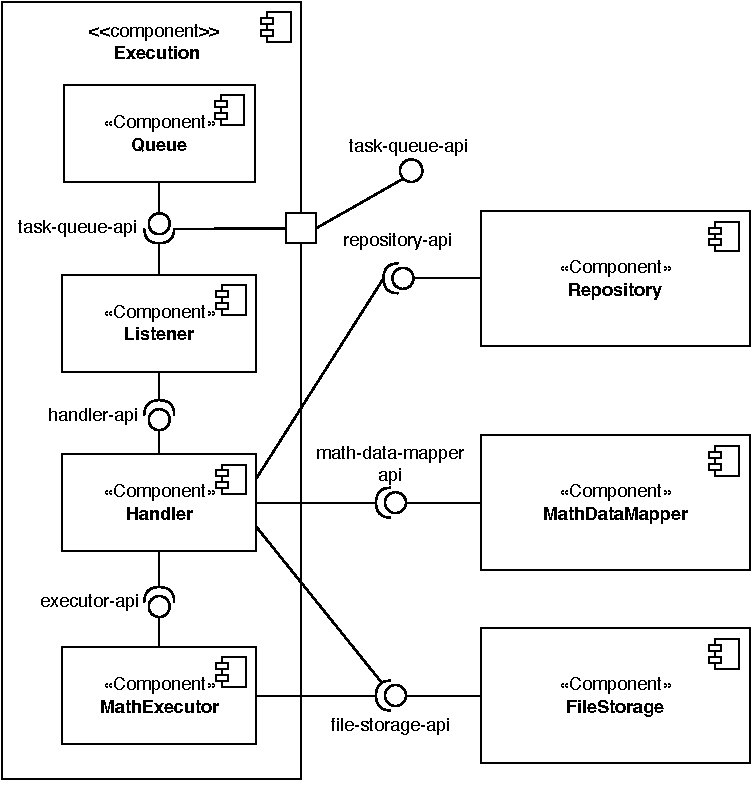
\includegraphics[scale=.5]{pictures/architecture/executor_component_detailed}
\end{figure}
\end{frame}


\begin{frame}
\frametitle{Хранилище расчётных данных}
\begin{figure}
    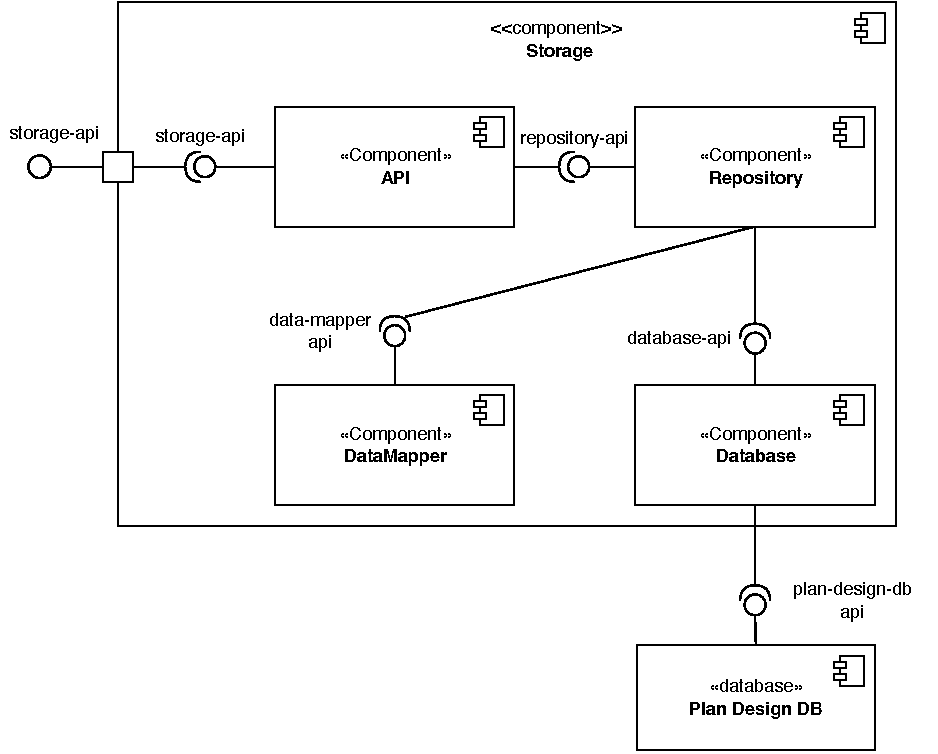
\includegraphics[scale=.55]{pictures/architecture/storage_component_common}
\end{figure}
\end{frame}

\begin{frame}
\frametitle{Сервис запуска расчётных задач}
\begin{figure}
    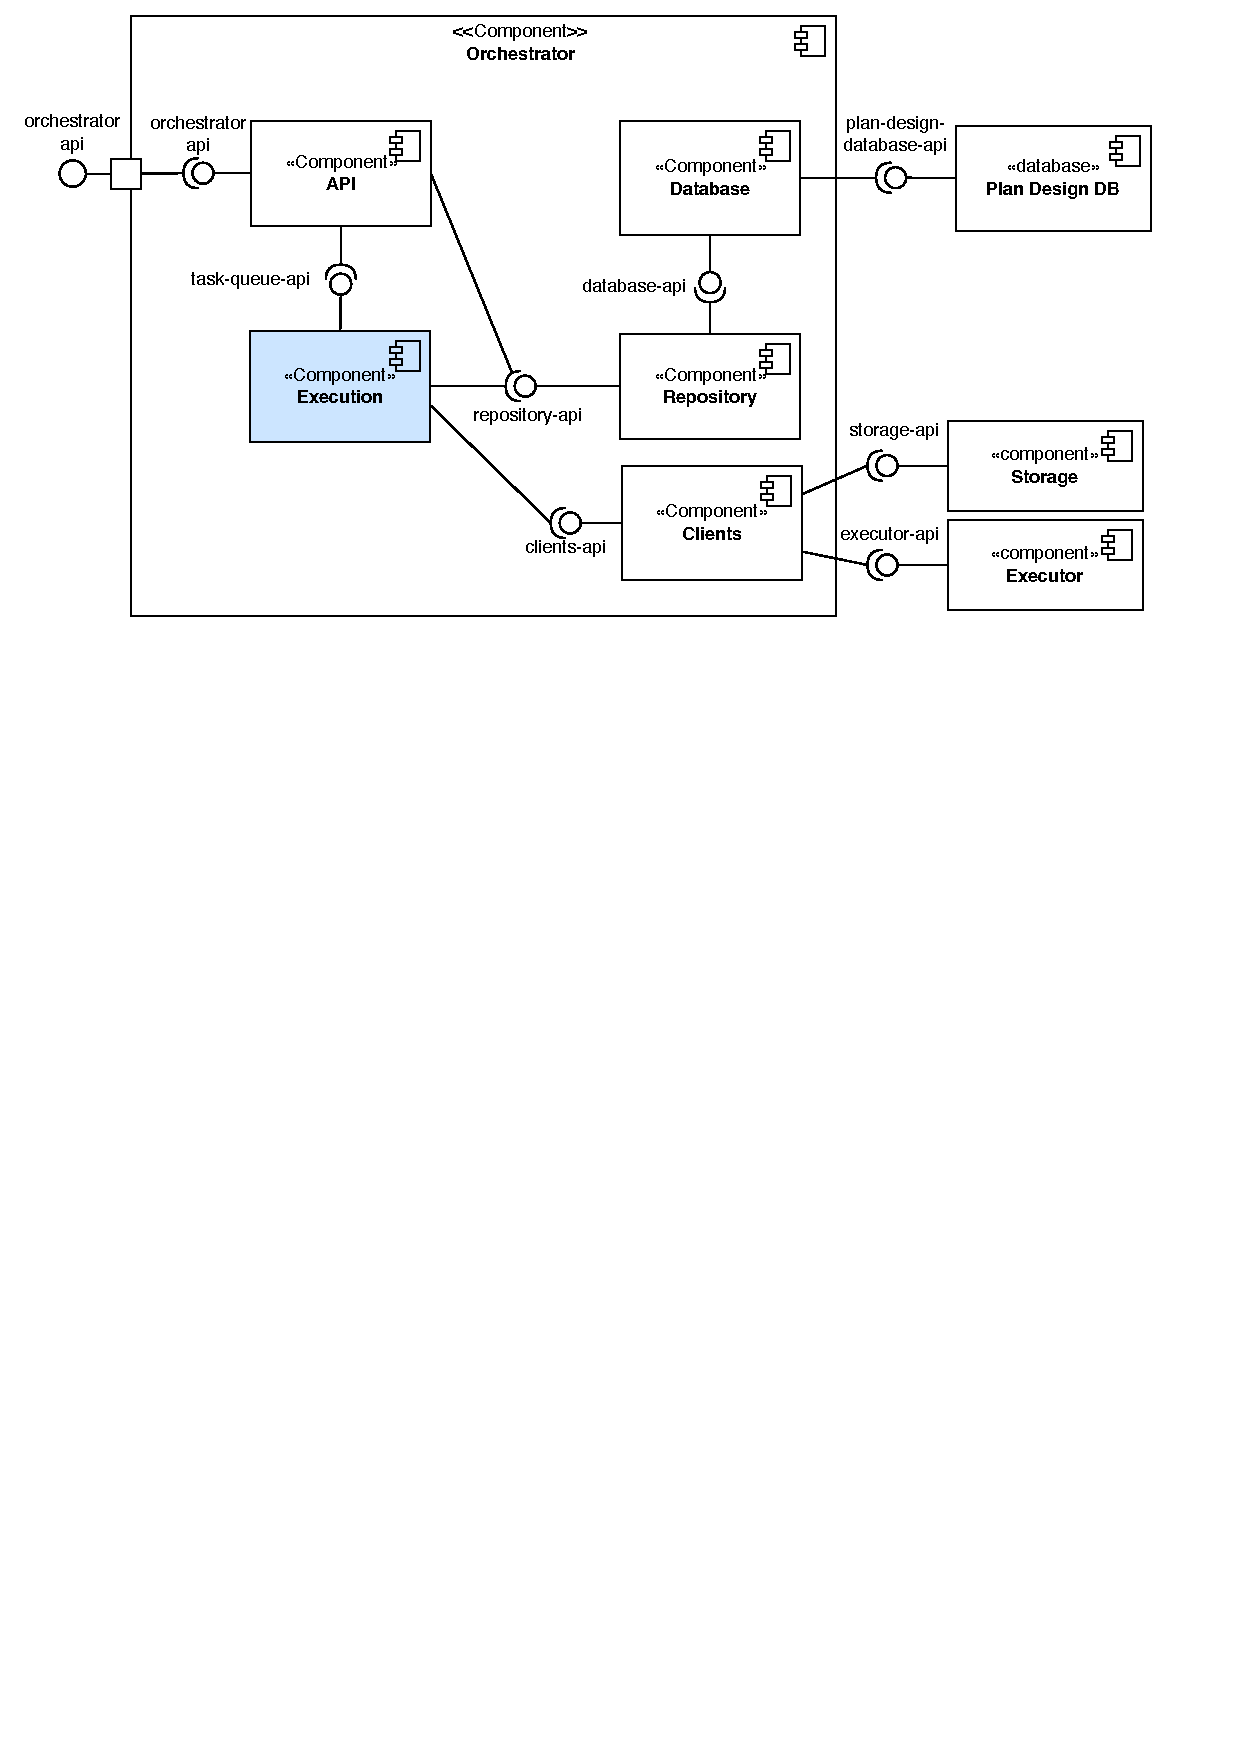
\includegraphics[scale=.5]{pictures/architecture/orchestrator_component_common}
\end{figure}
\end{frame}


\begin{frame}
\frametitle{Компонент запуска расчётных задач}
\begin{figure}
    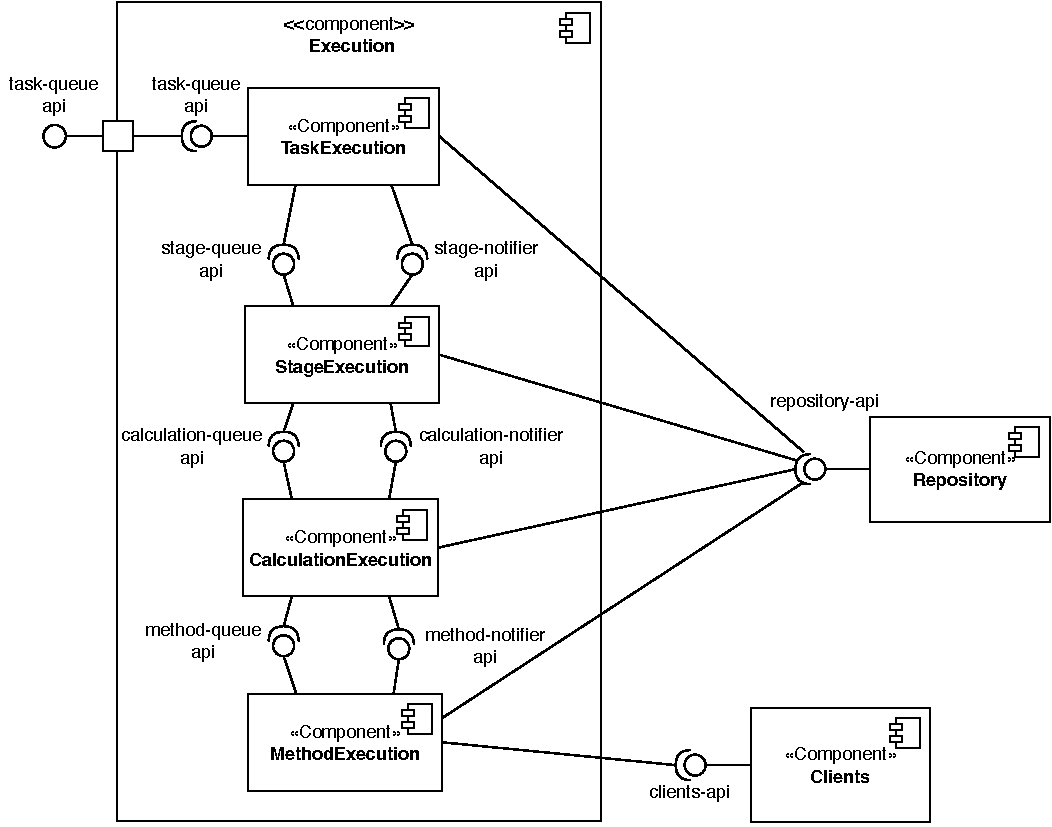
\includegraphics[scale=.5]{pictures/architecture/orchestrator_component_detailed}
\end{figure}
\end{frame}


\begin{frame}
\frametitle{Диаграмма последовательности запуска расчётных задач}
\begin{figure}
    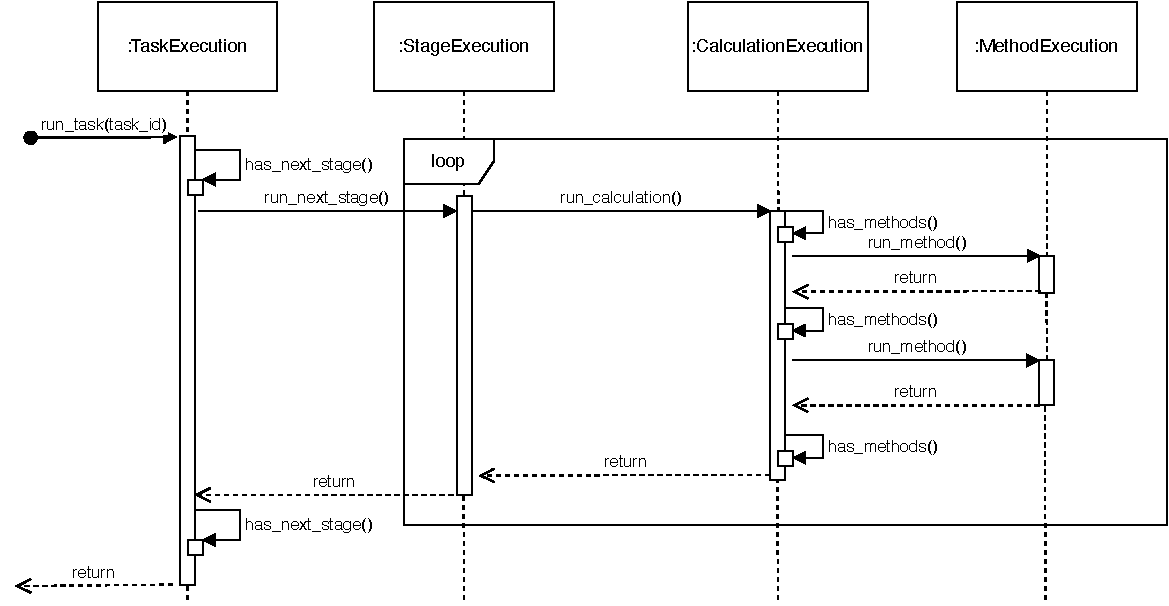
\includegraphics[scale=.7]{pictures/architecture/orchestrator_sequence}
\end{figure}
\end{frame}


\section{Программная архитектура}

\begin{frame}
\frametitle{Математическая библиотека}
\begin{figure}
    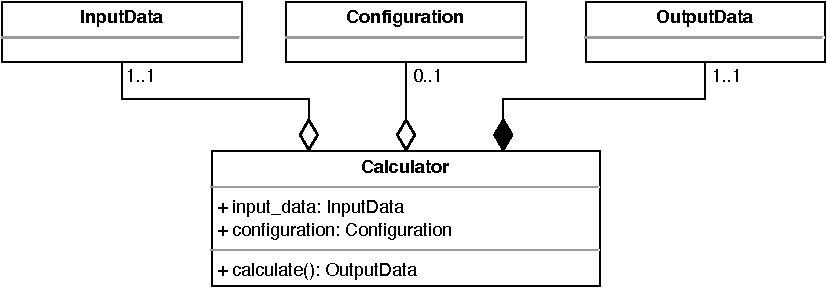
\includegraphics[scale=.8]{pictures/architecture/math_classes}
\end{figure}
\end{frame}

\begin{frame}
\frametitle{Расчётная модель данных}
\begin{figure}
    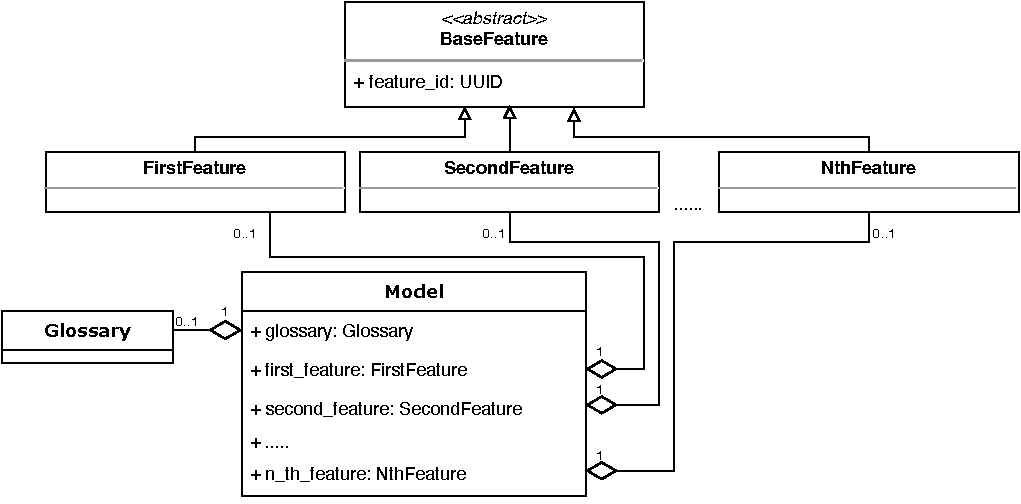
\includegraphics[scale=.7]{pictures/architecture/model_classes}
\end{figure}
\end{frame}
